% do not change these two lines (this is a hard requirement
% there is one exception: you might replace oneside by twoside in case you deliver 
% the printed version in the accordant format
\documentclass[a4paper, 11pt,titlepage,oneside,openany]{book}
\usepackage{times}


\usepackage{graphicx}
\usepackage{latexsym}
\usepackage{amsmath}
\usepackage{amssymb}
\usepackage{subfigure}
\usepackage{verbatim}
\usepackage{listings}
\usepackage{courier}
\usepackage{caption}
\lstset{
	language=Python,
	basicstyle=\small,
	numbers=left,
	numberstyle=\tiny,
	frame=tb,
	columns=fullflexible,
	showstringspaces=false,
	breaklines=true,
}
\usepackage{booktabs} 
\usepackage{glossaries}          
\usepackage{ntheorem}
\DeclareCaptionType{code}[Algorithm][List of Code] 
% \usepackage{paralist}
\usepackage{tabularx}
\usepackage{amsmath}
% this packaes are useful for nice algorithms
%\usepackage{algorithm}%;, algorithmic}
\usepackage[linesnumbered,ruled,vlined]{algorithm2e}
\SetKwInput{KwIn}{Input}                % Set the Input
\SetKwInput{KwOut}{Output}              % set the Output
%\AtBeginEnvironment{algorithm}{\scriptsize}
\AtBeginEnvironment{tabular}{\scriptsize}
\AtBeginEnvironment{amsmath}{\scriptsize}
%\usepackage{algorithmic}
\usepackage{array}
\usepackage{multirow}
\usepackage{url}
\urlstyle{same}

\newcommand\MyBox[2]{
	\fbox{\lower0.75cm
		\vbox to 1.7cm{\vfil
			\hbox to 1.7cm{\hfil\parbox{1.4cm}{#1\\#2}\hfil}
			\vfil}%
	}%
}

% well, when your work is concerned with definitions, proposition and so on, we suggest this
% feel free to add Corrolary, Theorem or whatever you need
\newtheorem{definition}{Definition}
\newtheorem{proposition}{Proposition}


% its always useful to have some shortcuts (some are specific for algorithms
% if you do not like your formating you can change it here (instead of scanning through the whole text)
%\renewcommand{\algorithmiccomment}[1]{\ensuremath{\rhd} \textit{#1}}
\def\MYCALL#1#2{{\small\textsc{#1}}(\textup{#2})}
\def\MYSET#1{\scshape{#1}}
\def\MYAND{\textbf{ and }}
\def\MYOR{\textbf{ or }}
\def\MYNOT{\textbf{ not }}
\def\MYTHROW{\textbf{ throw }}
\def\MYBREAK{\textbf{break }}
\def\MYEXCEPT#1{\scshape{#1}}
\def\MYTO{\textbf{ to }}
\def\MYNIL{\textsc{Nil}}
\def\MYUNKNOWN{ unknown }
% simple stuff (not all of this is used in this examples thesis
\def\INT{{\mathcal I}} % interpretation
\def\ONT{{\mathcal O}} % ontology
\def\SEM{{\mathcal S}} % alignment semantic
\def\ALI{{\mathcal A}} % alignment
\def\USE{{\mathcal U}} % set of unsatisfiable entities
\def\CON{{\mathcal C}} % conflict set
\def\DIA{\Delta} % diagnosis
% mups and mips
\def\MUP{{\mathcal M}} % ontology
\def\MIP{{\mathcal M}} % ontology
% distributed and local entities
\newcommand{\cc}[2]{\mathit{#1}\hspace{-1pt} \# \hspace{-1pt} \mathit{#2}}
\newcommand{\cx}[1]{\mathit{#1}}
% complex stuff
\def\MER#1#2#3#4{#1 \cup_{#3}^{#2} #4} % merged ontology
\def\MUPALL#1#2#3#4#5{\textit{MUPS}_{#1}\left(#2, #3, #4, #5\right)} % the set of all mups for some concept
\def\MIPALL#1#2{\textit{MIPS}_{#1}\left(#2\right)} % the set of all mips



\makeglossaries

\begin{document}

\pagenumbering{roman}
% lets go for the title page, something like this should be okay
\begin{titlepage}
	\vspace*{2cm}
  \begin{center}
   {\Large Hyperpartisan News Detection\\}
   \vspace{2cm} 
   {Bachelor Thesis\\}
   \vspace{2cm}
   {presented by\\
    Larissa Strauch \\
    Matriculation Number 1518629\\
   }
   \vspace{1cm} 
   {submitted to the\\
    Data and Web Science Group\\
    Prof.\ Dr.\ Ponzetto\\
    University of Mannheim\\} \vspace{2cm}
   {July 2019}
  \end{center}
\end{titlepage} 

% no lets make some add some table of contents
\tableofcontents
\newpage

\listofalgorithms
\listoffigures

\listoftables

\newglossaryentry{tf}
{
	name=TF,
	description={Term Frequency}
}
\newglossaryentry{idf}
{
	name=IDF,
	description={Inverse Term Frequency}
}
\newglossaryentry{tfidf}
{
	name=TF-IDF,
	description={Term Frequency-Inverse Term Frequency}
}
\newglossaryentry{bert}
{
	name=BERT,
	description={Bidirectional Encoder Representations from Transformers}
}
\newglossaryentry{cbow}
{
	name=CBOW,
	description={Continous Bag of Words}
}
\newglossaryentry{mnb}
{
	name=Multinomial NB,
	description={Multinomial Naives Bayes}
}
\newglossaryentry{rnn}
{
	name=RNN,
	description={Recurrent Neural Network}
}
\newglossaryentry{lstm}
{
	name=LSTM,
	description={Long Short-Term Memory}
}
\newglossaryentry{mlm}
{
	name=MLM,
	description={Masked LM}
}
\newglossaryentry{nlp}
{
	name=NLP,
	description={Natural Language Processing}
}
\newglossaryentry{use}
{
	name=USE,
	description={Universal Sentence Encoder}
}
\newglossaryentry{elmo}
{
	name=ELMo,
	description={Embeddings from Language Models}
}
\printglossaries %in cmd for printing: makeindex -s BA.ist -t BA.glg -o BA.gls BA.glo

% evntuelly you might add something like this
% \listtheorems{definition}
% \listtheorems{proposition}

\newpage


% okay, start new numbering ... here is where it really starts
\pagenumbering{arabic}

\chapter{Introduction}
In the digital age it is possible to access news and information anytime and anywhere. Above all, freedom of press makes it possible for everyone to express his or her opinion publicly. Many people who read news nowadays assume that the information presented is correct and neutral. Unfortunately, this is very often not the case. Especially in special political situations, even supposedly trustworthy news portals are not always neutral.  Thus, the website \textit{adfontesmedia} \footnote{https://www.adfontesmedia.com/} shows, on basis of Media Bias Charts, that even well-known news portals, such as Fox News or the New York Times, show partly extreme/unfair interpretations of the news. The most interesting question here is what is hyperpartisan and how hyperpartisan articles can be recognized. For example, a study by the Knight Foundation \cite{study} describes that the perceived trustworthiness of news content depends on how the news source is viewed.  This means that left-wing political supporters, would be less likely to call a newspaper article from a left-wing publisher hyperpartisan than right-wing supporters. This raises the question, however, when people are not sure, if an article is hyperpartisan, how this should be recognized at all and how it could be tackled.  \\
\indent Hyperpartisan is defined as "extremely partisan; extremely biased in favor of a political party". Such a biased attitude towards a particular party often leads to the output of fake news. Especially lately fake news have been in discussion. Fake news are defined as "false stories that appear to be news, spread on the internet or using other media, usually created to influence political views or as a joke". According to Webster's Dictionary, their beginnings date back to 1980 \cite{webster}, but they first attracted a lot of attention in April 2017 when Facebook Inc. published a whitepaper stating that their platform was being used for targeted disinformation campaigns \cite{facebook}. This was expressed, among other things, in social bots \cite{socialbots}, which are computer programs that have been increasingly used in social networks in recent years to spread fake news. It is even more difficult to distinguish fake news from normal news than to recognize hyperpartisan articles. This is reflected in the fact that even professisonals cannot distinguish between true and fake news. To solve this problem, the first approach could be to detect hyperpartisan articles.  \\
\indent PANs "SemEval Task 4: Hyperpartisan News Detection" \cite{hyperpartisannewsdetection} takes up on this challenge by assigning the task to implement a program that automatically detects whether a newspaper article is hyperpartisan. The latest findings in data science and above all in Natural Language Processing (NLP) contribute to develop such a model. Since a computer, unlike humans, cannot draw on experience to better understand language, these algorithms and procedures must apply artificial intelligence and machine learning. \gls{nlp}, therefore, deals with techniques and methods for machines to process natural language. Since 1950 \gls{nlp} has been dealing with tasks like machine translation and information retrieval. Since then \gls{nlp} has gone through several developments. Among others, the development of Neural Language Models in 2001 \cite{neural}, Word Embeddings in 2013 \cite{wb1}, Sequence-to-Sequence Models in 2014 \cite{s2s} and pre-trained models in 2018 \cite{pre1}\cite{pre2}\cite{pre3} are of particular importance. \\
\indent In the context of this bachelor thesis I will discuss how a program based on SemEvalTask 4 can be implemented. I will use classical methods of text classification as well as the latest development in \gls{bert} \cite{bert}. Within the framework of classical approaches, I will discuss classical approaches for text presentation using Word Embeddings and the \gls{tfidf}  \cite{infor} measure, which I will set in relation to \gls{bert} embeddings, which represent a new kind of model using a bidirectional learning process. In addition to the question of which techniques can be used to identify a program for detecting hyperpartisan articles, this also raises the question of whether \gls{bert} Embeddings improve the performance of a model compared to classical methods. \\
\indent Therefore, in the first chapter of this thesis I will deal with the mathematical basics of the methods used here, whereupon I will describe the data available to me in the second chapter. Chapter 3 describes the procedure to implement such a program. Chapter 4 refers to the evaluation of the different classification procedures before a conclusion is drawn in \textit{Chapter 5}. 

\chapter{Related Work}
Different classifiers were designed in the context of SemEval Task 4. For this purpose, the most common were Neural Networks, but overall all kinds of classifiers were used. 
\indent The winners of the competition used a model based on \gls{elmo} \cite{elmo}. \gls{elmo} was designed by AllenNLP in 2018 and uses a deep, bidirectional LSTM model to design character-based word representations. The advantage is that the employment of character embeddings makes it possible to identify morphological features which word-level embedding might overlook. Additionally, this ensures that valid word representations can be formed even for out-of-vocabulary words. The winners use a pre-trained \gls{elmo} model to output three vectors for each word. They state, that each vector corresponds to a layer output of the pre-trained \gls{elmo} model, whereupon they calculate the average of all three vectors to create the last word vector. Finally, the sentence vector is calculated by averaging the word vectors of a sentence. The complete development of their model was presented in the paper "Team Bertha by Suttner at SemEval-2019 Task 4: Hyperpartisan News Detection using \gls{elmo} Sentence Representation Convolutional Network" \cite{gewinner}. With their model they achieved an accuracy score of 0.822, a precision score of 0.871, a recall score of 0.755 and an F1 score of 0.809 on the by-Article dataset. \footnote{bertha-von-suttner - GitHub Repsoritory: https://github.com/GateNLP/semeval2019-hyperpartisan-bertha-von-suttner/tree/4b1d74b73247a06ed79e8e7af30923ce6828574a} \\
\indent Team Vernon Fenwick used a combination of handcrafted text features and models that capture semantics to represent an article. Here the authors say that the handcrafted text features capture the tone, over praise, and mood in an article. For these text features a Bias Score, Article Level Polarity, Sentence Level Polarity, Subjectivity \& Modality and Superlatives \& Comparatives were used. The complete functionality of these features can be viewed in their paper "Vernon-fenwick at SemEval-2019 Task 4: Hyperpartisan News Detection using Lexical and Semantic Features" \cite{vernon}. For the semantic features, they used Glove \cite{glove}, Doc2Vec \cite{doc2vec}, and Universal Sentence Encoder (USE) \cite{use}, with the USE giving the best score in conjunction with the hand-made features. 
\newpage 
\noindent Overall, the group came in second with an Accuracy Score of 0.820, a Precision Score of 0.815, a Recall Score of 0.828, and an F1 Score of 0.821. \\
\indent A third group also used \gls{bert} embeddings. They had a different approach than the one used in this thesis. They did not use the provided pre-trained models of \gls{bert}, but did the pre-training based on the large by-Publisher dataset and fine-tuned based on the ones labeled by-Article. The complete procedure, as well as any anomalies during the development of the classifier, can be found in the paper "Harvey Mudd College at SemEval-2019 Task 4: The Clint Buchanan Hyperpartisan News Detector" \cite{bertgruppe}. In total, they achieved 10$^{th}$ place with their approach with an accuracy score of 0.771, a precision score of 0.832, a recall score of 0.678 and an F1 score of 0.747. \footnote{Clint Buchanan - GitHub Repsoritory: https://github.com/hmc-cs159-fall2018/final-project-team-mvp-10000/tree/c9da670b8a39068aa2d3154023ea44e-0b1266b7d}. \\
\indent A complete overview of the task definition, used classifiers and participants can be found in the paper "SemEval-2019 Task 4: Hyperpartisan News Detection" organized by the publishers \cite{hyperpartisannewsdetection}.


\chapter{Fundamentals}
\section{Text Representation}
\subsection{Term Frequency-Inverse Document Frequency}
\indent Term frequency (\gls{tf}) is a measure that denotes how frequently a term \textit{t} appears a the document \textit{d}. One way to compute \gls{tf} is \cite{IR-book}:\\
\[
tf(t,d)=\frac{1+\log(tf_{t,d})}{1+\log(ave_{t\in d}(tf_{t,d}))}
\]
Where $1+\log(tf_{t,d})$ reflects how many times the term $t$ appears in document $d$ and $1+\log(ave_{t\in d}(tf_{t,d}))$ is the highest occurrence of any term in document $d_i$.\\

\indent Inverse Doucment Frequency (\gls{idf}) points to the assumption that the informativeness of the term \textit{t} is inversely proportional to the number of documents in the collection in which the term appears \cite{IR-book}.\\
\[
idf(t_i)=log\frac{N}{d \in D : t \in d}
\]
Here $N$ is the total amount of doucments in a document set and $d \in D : t \in d$ is the amount how many times the term $t$ appears in the document set.\\

\indent To compute the weight for the term $t_i$ within the document $d_j$ we simply multiply the \textit{TF} and \textit{IDF} components:
\[
w_{ij}=tf(t_i, d_j)\cdot idf(t_i)
\]
\indent The more often a word occurs in the document, the higher the \gls{tfidf} value, which is compensated by calculating the frequency of the word in the corpus. This makes it possible to find a balance between words that usually occur frequently and words that usually do not.\\
\newpage
Therefore, \Gls{tfidf} indicates how significant a word is to a document in a collection or corpus. It is regularly used as a weighting factor in Information Retrieval and Text Mining. \Gls{tfidf} is easy to compute. In addition, it is possible to extract the most descriptive terms, as well as to calculate the similarity between tw terms. However, \gls{tfidf} is based on the bag-of-words (BoW) model \cite{distributionalhypothesis}, which is why it disregards aspects such as text position, semantics and co-occurrence.

\subsection{Word Embeddings}
\indent Word Embeddings are based on the approach of Harris' Distributional Hypothesis \cite{distributionalhypothesis} from 1951, which states, that words that occur in the same contexts tend to have similar meanings. \\
\indent A Word Embedding provides a word vector for each word. This is done by extracting features from that word within the context in which it appears and assigning it a place within the vector space. Two similar words will occupy locations near one another within this vector space, while words that differ will have positions much further apart. This makes it possible to perform distance calculation by computing cosine distance. There are different models for learning word vectors. Among others fastText \cite{fasttext}, GloVe \cite{glove} and word2vec. \\

%\subsubsection{Word2Vec}
Word2Vec is a "2-Model Architecture for computing continuous vector representations of words from very large dataset"\cite{effiecientestimation} that creates an n-dimensional vector space in which each word is represented as a vector. Word2Vecs 2 learning models are the \gls{cbow} and Skip-Gram-Model.\\
\noindent \gls{cbow} uses the context word to predict the target word. The input is a one-hot encoded vector. The weights between the input layer and the output layer can be represented by a $V \cdot N$ matrix \textit{W} where "each row of $W$ is the $N$-dimension vector representation $w_v$ of the associated word of the input layer" \cite{word2vecparam}. The hidden-layer \textit{h} is computed by multiplying the one-hot encoding vector of the input word $w_I$ with the weight matrix \textit{W} \cite{word2vecparam}.
\[
h=W^Tx=W_{(k, \cdot)}^{T}:=v_{w_I}^{T}
\] 
Next there is another weight matrix $W'={w'_{ij}}$ which is an $N \cdot V$ matrix. With these weights it is finally possible to compute a score $u_j$ for each word in the vocabulary \cite{word2vecparam}
\[
u_{j}={v'}_{w_j}^{T}h
\] where ${v'}_{w_j}$ is the \textit{j}-th column of the matrix \textit{W'}. \\
\newpage
\noindent Afterwards the \textit{softmax} function is used, "which is a log-linear classification model, to obtain the posterior distribution of words" \cite{word2vecparam}.
\[
p(w_j|w_I)=y_j=\frac{exp(u_j)}{\sum_{j'=1}^V exp(u_{j'})}
\] 
\indent In contrast to the \gls{cbow} model,  Skip-Gram uses the target word to predict the context words. The input stays a one-hot encoding vector, the hidden layers definition stays the same as in the \gls{cbow} model, each output is still using the same hidden layer to output matrix as in the \gls{cbow} model $p(w_{c,j}=w_{O,c}|w_I)=y_{c,j} = p(w_j|w_I)=y_j$ and the function for $u_j=u_{c,j}$ stays the same \cite{word2vecparam}. However, in the output layer is now outputting \textit{C} multinomial distributions.  

\section{Classification Methods}
Classification is about predicting a particular outcome based on given training data. For this prediction, a classification algorithm processes the training data set, which consists of a set of features and the respective predictions. The algorithm attempts to discover relationships between given features  of the instances and the associated classes to learn a function which makes it possible to predict the correct class based on the features of an instance. Thereafter, the algorithm receive a test dataset which it has not seen before. This dataset contains the same features as the training set but not the corresponding class names. With the previously learned function, the algorithm now assigns a class name to each instance  of the test record. \\
\subsection{Multinomial Naive Bayes Classifier}
The Naive Bayes classifier is based on  Bayes' theorem \cite{btheory}, which comes from the probability calculus and describes the calculation of conditional probability. Each object in this classification approach is assigned to the class for which the highest probability was computed or for which the lowest costs arise in this assignment.  \\
\noindent The Multinomial Naive Bayes classifier assumes that the position of the word does not matter, as well as  that the feature probabilities $Pr(t_i|c_)$ are independent given a class $c$.
The probability of a class value $c$ given a test document $t_i$ is computed as \cite{multinomialnb}
\[
Pr(t_i|c)=(\sum_{n}f_{ni})!\prod_{n}\frac{Pr(w_n|c)^{f_{ni}}}{f_{ni}!}
\]
where $f_{ni}$ is the number of times a word $n$ appears in document $t$ and $Pr(t_i|c)$ is the probability of detecting word $n$ given class $c$.
\newpage
\subsection{Logistic Regression Classifier}
\noindent Like Naive Bayes, Logistic Regression is a probabilistic classifier, and ,thus, classifies by estimating the probability $P(Y|X)$ that the object belongs to a particular class.
It can be derived analogously to the linear regression model \cite{logisticregressionbook}, 
\[
P(Y|X)=Pr(Y=1)=X\beta
\]
where $X$ is the vector of predictors $\{X_1,...,X_n\}$ and $\beta$ is the model's parameter vector. In contrast to linear regression, in logistic regression only values between 0 and 1 are obtained, which can be attributed to the addition of the sigmoid function $p(\bar{x}_i)=\sigma(\bar{x}_i)=\frac{1}{1+e^{-z_i}}$ \cite{algorithms2}, where $z_i=\log(\frac{p(\bar{x}_i)}{1-p(\bar{x}_i)})$. \\
So, if the probability distribution is modelled with a sigmoid, the following is obtained \cite{algorithms2}:
\[
z_i=\log(\frac{p(\bar{x}_i)}{1-p(\bar{x}_i)})=\log(\frac{\frac{1}{1+e^{-z_i}}}{1-\frac{1}{1+e^{-z_i}}})=\log(\frac{1}{e^{-z_i}})=z_i
\]
This opens up the possibility of defining the probability that a sample belongs to a class \cite{algorithms2}:
\[
p(y|\bar{x}_i)=\sigma(\bar{x}_i,\bar{\Theta})
\]
where $\Theta$ is a single parameter vector.
\noindent To find the optimal $\Theta$ by which $p(y|\bar{x}_i)$ gets close to 0 or 1, the log-likelihood is maximized relying upon the output class. Therefore the optimization problem can be expressed, utilizing the indicator notion as the minimization of the loss function \cite{algorithms}:
\[
l(\Theta)=-\sum_{i}y_i\log(\sigma(z_i))+(1-y_i)\log(1-\sigma(z_i))
\]

\noindent This implies, if $y=0$, the first term ends up $0$ and the second $\log(1-\sigma(z_i)$, which results in a log-likelihood of $0$. In the event that $y=1$, the second term ends up 0 and the first one corresponds to the log-likelihood of $z$. Along these lines, both cases are integrated into a solitary articulation. \\
\\ A major issue in machine learning is the aspect of overfitting. Overfitting tends to adjust the model too much to the training data. This happens when a model learns the details in the training data so that the performance of the model is contrarily influenced by new data. This implies that noise or random fluctuations in the training data are recorded and learned as concepts by the model. The issue is that these concepts do not apply to new data and negatively impact the generalization of the model. Therefore, there is the process of \textit{regularization}, which is a form of regression that decreases the coefficient estimation to $0$ and assumes that smaller weights generate simpler models and thus helps avoid overfitting. \\
\noindent Two of the most commonly used regularization techniques are \textit{Lasso Regression (L1)} and \textit{Ridge Regression (L2)}, which differ mainly in the penalty term. \\
\noindent The \textit{L1} loss function minimizes the sum of the absolute differences between the target value and the estimated values. If input characteristics have weights closer to zero, this results in a sparse L1 standard. In the Sparse solution, most of the input features have zero weights and very few features have non-zero weights. The L1 regulation offers a function selection. This is done by associating insignificant input features with zero weights and useful features with a non-zero weight. 
\noindent \textit{L1} solves the regularized logistic regression by minimizing the following cost function:
\[
\min_{w, c} \quad \|w\|_1 + C \sum_{i=1}^n \log(\exp(1+e^{-y_ix^Tx_i})
\]
whereas \textit{L2} solves it the following way:
\[
\min_{w, c} \quad \frac{1}{2}w^T w + C \sum_{i=1}^n \log(1+e^{-y_iw^Tx_i})
\]
Here, $C>0$ is the penalty parameter, $w$ is the vector, $w^T$ is an additional dimension, $x_i$ is an instance of the vector and $y_i$ is an instance label pair $\in \{-1,+1\}$ \cite{liblinear}.\\
The L2 loss function is essentially about minimizing the sum of the square of the differences between the nominal value and the estimated values.
L2 control forces the weights to small weights, but does not make them zero and leads to a not sparse solution. In addition, L2 is not robust against outliers, since square terms inflate the error differences of the outliers and the regularization term tries to correct them by punishing the weights.


\subsection{Decision Trees and Random Forest Classifier}
\subsubsection{Decision Trees}
Starting from the root node of a tree, a feature is evaluated from which a branch is subsequently selected. This process is repeated until the last node in the tree (leaf) is reached, which supplies the corresponding class. Different approaches have been developed in decision trees. One of the first is called \textit{Iterative Dichotomizer (ID3)}. However, this algorithm had the disadvantage that explicit functions were necessary, which led to the development of C4.5. Like ID3, C4.5 manages continuous values. In return to ID3, C4.5 could furthermore manage summarized and decreed values and transform a tree into a set of conditional expressions. Nevertheless, the most recent development called CART (Classification and Regression Trees) was introduced, which allows the use of absolute and numeric values, as well as the non-use of standard sets. In addition, CART trees can be utilized for characterization and fallback assignments. \cite{algorithms2}\\
\noindent The algorithm uses impurity measures to select a particular branch from a leaf. Among others, the two most common measures are \textit{Gini Impurity} and \textit{Cross Entropy} Index \cite{algorithms}. 
\newpage
\noindent These impurity measures are  applied to each candidate subset, and the resulting values are combined (e.g., averaged) to provide a measure of the quality of the split,
\[
I_{Gini}(j)=\sum_{i}p(i|j)(1-p(i|j))
\]
\[
I_{Cross-entropy}(j)=-\sum_{i}p(i|j)log(p(i|j))
\]
where $j$ is a certain node, $p(i|j)$ is the probability with $i \in [1,n]$ associated with each class.\\
\noindent The \textit{Gini} Index measures how often a randomly selected element from the set would be mislabeled if it has been randomly chosen according to the distribution of labels in the subset. The minimum index (0,0) is achieved when all examples are classified into a solitary class.\\
\noindent "\textit{Cross-Entropy} is based on information theory, and assumes null values only when samples belonging to a single class are present in a split, while it is maximum when there's a uniform distribution among classes. This index is very similar to the Gini impurity, even though, more formally, the cross-entropy allows to select the split that minimizes the uncertainty about the classification, while the \textit{Gini} impurity minimizes the probability of misclassification" \cite{algorithms}.

\subsubsection{Random Forest Classifier}
The Random Forest classifier is a classification technique that creates multiple decision trees from randomly selected subsets of training data. Each tree in this process may make a decision, these votes are then aggregated to determine the final class. According to Breiman \cite{randomforest} the Random Forest algorithm is as follows:\\

\begin{algorithm}[H]
	\DontPrintSemicolon
	Set the number of decision trees $N_c$\;
	\For{$i\gets 1$ \KwTo $N_c$}
		{Create a dataset $D_i$ sampling with replacements from the original dataset $X$}
	Set the number of features  to consider during each split $N_f$\;
	Set an impurity measure\;
	Define an optimal maximum for each tree\;
	\For{$i\gets 1$ \KwTo $N_c$}
		{Random Forest: Train the decision tree $d_i(x)$ using the dataset $D_i$ and selecting the best split among \textit{Nf} features randomly sampled \\
		Extra-trees:  Train the decision tree $d_i(x)$ using the dataset $D_i$ computing before each split $n$ random thresholds and selecting the one that yield the least impurity}
	Define an output function averaging the single outputs or employing a majority vote
	\caption{Random Forest}
\end{algorithm}

\newpage
\subsection{Bidirectional Encoder Representation from Transformers}
Bidirectional Encoder Representations from Transformers (\gls{bert}) \cite{bert} is a novel model that was introduced in October 2018 by researchers at Google AI Language and has since caused a stir in the field of machine learning by representing state-of-the-art results in a variety of Natural Languag Processing tasks. The special feature of this model, unlike previous efforts, is the technical innovation of bidirectional training of transformers. \\
\noindent In order to understand how the actual model, and thus the classification model applied in this thesis, I will discuss the basics and the actual \gls{bert} model in the following section.

\subsubsection{Transfer Learning}
\textbf{Recurrent Neural Networks}
\begin{figure}[h]
	\centering
	%PC:
	%\includegraphics[width=0.7\linewidth]{C:/Users/Laris/Documents/Bachelorarbeit/Git/ThesisPaper/Pictures/rnn.png}
	%Lap Top:
	\includegraphics[width=0.8\linewidth]{C:/Users/Larissa/Documents/Uni/Bachelorarbeit/Git/ThesisPaper/Pictures/rnn.png}
	\caption{\gls{rnn} and Feedforward Neural Network \cite{rnn}}
\end{figure}\\
Recurrent Neural Networks (\gls{rnn}) are a kind of artificial neural network, which considers time and order. Unlike Feedforward algorithms \cite{feedforward}, which use only the current example as input, \gls{rnn}s also use the Input Example, which they perceived in previous steps (Figure 3.1). 
This sequential information is retained over many time steps in the hidden state of the RNN as it cascades forward to affect the processing of each new example. This means that the RNN finds correlations between events that are separated by many steps. These relationships are referred to as \textit{long-term dependencies} because a subordinate event is dependent on one or more preceding events.\\
\newpage
\noindent Mathematically, a \textit{simple recurrent neural network} \cite{ELMAN1990179} can be represented as follows \cite{rnnmodel}:
\[
x(t)=w(t)+s(t-1)
\]
\[
s_j(t)=f(\sum_{i}x_i(t)u_{ji})
\]
\[
y_k(t)=g(\sum_{j}s_j(t)v_{kj})
\]
Where $x(t)$ is the input, $s(t)$ the hidden and $y(t)$ the output layer. $s_t$ is the function of the input at the same time step $t$, modified by a weight matrix $w$, which has been added to the hidden state's previous step $s(t-1)$ and multiplied by its own hidden-state-to-hidden-state matrix $u$. The weight matrices $w$ and $u$ are filters that determine the importance of matching the current input as well as the past hidden-state. These generate errors which return via backpropagation and are used to adjust their weights until the error can no longer be reduced. The sum of the weight input and hidden state is squashed by the functions $f$ or $g$, where  $f(z)$ represents the sigmoid function
\[
f(z)=\frac{1}{1+e^{-z}}
\]
and $g(z)$ the softmax function
\[
g(z_m)=\frac{e^{zm}}{\sum_{l}e^zk}
\]
The initial value $s(0)$ can take the values 0 or 1, whereas in all further steps $s(t+1)=s(t)$. \\
\noindent A problem of \gls{rnn}s is the disappearance and explosion of the gradient. Since the layers and time steps of deep neural networks are wired together by multiplication, derivatives are susceptible to disappearance or explosion. With an exploding gradient, the weights at the upper end become saturated, whereas with disappearing gradients, the final value will tend to 0. \\

\noindent \textbf{Long Short-Term Memory} \\
\begin{figure}[h]
	\begin{minipage}[b]{0.4\linewidth}
		%PC:
		%\includegraphics[width=0.8\linewidth]{C:/Users/Laris/Documents/Bachelorarbeit/Git/ThesisPaper/Pictures/inputg.png}
		%Lap Top:
		\includegraphics[width=0.8\linewidth]{C:/Users/Larissa/Documents/Uni/Bachelorarbeit/Git/ThesisPaper/Pictures/inputg.png}
		\caption{Input gate$_1$ \cite{rnn}}
	\end{minipage}
	\hfill
	\begin{minipage}[b]{0.4\linewidth}
		%PC:
		%\includegraphics[width=0.8\linewidth]{C:/Users/Laris/Documents/Bachelorarbeit/Git/ThesisPaper/Pictures/inputg2.png}
		%Lap Top:
		\includegraphics[width=0.8\linewidth]{C:/Users/Larissa/Documents/Uni/Bachelorarbeit/Git/ThesisPaper/Pictures/inputg2.png}
		\caption{Input gate$_2$ \cite{rnn}}
	\end{minipage}
	\begin{minipage}[b]{0.4\linewidth}
		%PC:
		%\includegraphics[width=0.8\linewidth]{C:/Users/Laris/Documents/Bachelorarbeit/Git/ThesisPaper/Pictures/forgetg.png}
		%Lap Top:
		\includegraphics[width=0.8\linewidth]{C:/Users/Larissa/Documents/Uni/Bachelorarbeit/Git/ThesisPaper/Pictures/forgetg.png}
		\caption{Forget gate \cite{rnn}}
	\end{minipage}
	\hfill
	\begin{minipage}[b]{0.4\linewidth}
		%PC:
		%\includegraphics[width=0.8\linewidth]{C:/Users/Laris/Documents/Bachelorarbeit/Git/ThesisPaper/Pictures/outputg.png}
		%Lap Top:
		\includegraphics[width=0.8\linewidth]{C:/Users/Larissa/Documents/Uni/Bachelorarbeit/Git/ThesisPaper/Pictures/outputg.png}
		\caption{Output gate \cite{rnn}}
	\end{minipage}
\end{figure}
\indent Long Short-Term Memory (\gls{lstm}) units \cite{lstm} are a modification of the RNNs which represent a problem elimination for the disappearing gradient. Unlike standard RNNs, \gls{lstm}s no longer consist of a single neural network layer but of four. \gls{lstm}s are formed by multiple gates which close and open (Figure 5.2 - 5.5). This allows a cell to make decisions about what to back up and when to read, write or delete. Within a cell, information can be saved, written or read. Gates act on the signals they receive and block or route the data they filter with their own weights based on their strength and import. These weights are tailored via the learning process of the recurring networks. 
\newpage 
\noindent This means that cells learn when to enter, leave or remove facts by iteratively making assumptions, propagating errors backwards and adapting weights via gradient descent.\\
The different gates of \gls{lstm}s are the Input, Forget and Output Gates, where the Input Gate controls the contribution of a new input to the memory, the Forget Gate controls the limits up to which a value remains in the memory and the Output Gate controls the limit up to which the memory in the activation block of the output contributes. Mathematically, the different gates can be represented as follows \cite{rnn}: 
\begin{itemize}
	\item Input Gate - Figure 5.2: 
	\begin{itemize}
		\item $i_t=\sigma(W_i \cdot [h_{t-1}, x_t]+b_i)$
		\item $\acute{C}=\tanh(W_C \cdot [h_{t1}, x_t]+b_c)$
		\item where $x_t$ is the time step at $t$, $h_{t-1}$ denotes the hidden state at time step $t-1$, $i_t$ is the input gate layer output at step $t$, $\acute{C}$ refers to candidate values to be added to the input gates output at time $t$, $b_i$ and $b_c$ denote the bias for the input gate layer and the candidate value computation and $W_i$ and $W_c$ denote the weights for the input gate layer and the candidate value computation.
	\end{itemize}	
	\item  Input Gate - Figure 5.3:
	\begin{itemize}
		\item $C_t=f_t*C_{t-1}+i_t*C_t$
		\item Where $C_i$ denotes the cell state after time step $i$ and $F_t$ is the forget state at step $t$.
	\end{itemize}
	\item Forget Gate - Figure 5.4:
	\begin{itemize}
		\item $f_t=\sigma(W_f \cdot [h_{t-1}, x_t]+b_f)$
		\item Where $f_t$ denotes the forget state at time step $t$ and $W_f$ and $b_f$ are the weights and bias for the forget state at step $t$.
	\end{itemize}
	\item Output Gate - Figure 5.4:
	\begin{itemize}
		\item $o_t=\sigma(W_o \cdot [h_{t-1},x_t]+b_o)$
		\item $h_t=o_t*\tanh(C_t)$
		\item Where $o_t$ is the output gate's output at time step $t$ and $W_o$ and $b_o$ denote the weights and bias for the output gate at time step $t$.
	\end{itemize}
\end{itemize}


\noindent "Today, \gls{lstm} networks have become a more popular choice than basic \gls{rnn}s, as they have proven to work tremendously on diverse sets of problems. Most remarkable results are achieved with \gls{lstm} networks than \gls{rnn}s, and now the phenomenon has extended such that wherever an \gls{rnn} is quoted, it usually refers to \gls{lstm} network only" \cite{rnn}.\\

\noindent \textbf{\gls{rnn} Encoder-Decoder} \\
\noindent Classic RNNs and LSTMs have the problem that the input and output length of the sequences may vary. This led to the development of the RNN Encoder-Decoder \cite{encodedecode}, which consists of 2 recurring neural networks that function as a pair of encoders and decoders. Here the encoder maps a variable length input sequence to a fixed length vector, whereupon the decoder maps the vector representation to a variable length output sequence. \textit{Cho et. al} states, that "the encoder is an \gls{rnn} that reads each symbol of an input sequence x sequentially. After finishing the reading process of a sequence, the hidden state of the \gls{rnn} is a summary c of the complete input sequence" \cite{encodedecode}. This means that, at the end of the training, the encoder provides an input feature vector that can be used by the decoder to construct the input with those aspects that are most essential to make the reconstructed input noticeable as the actual input. The paper also states, that the "decoder represents another \gls{rnn} that has been trained to generate the output sequence by predicting the next symbol $y_t$ under the condition of the hidden state $h_t$. In contrast to typical \gls{rnn}s, $y_t$ and $h_t$ are also dependent on each other by $y_{t-1}$ and the combination c in this case". 
\newpage
\noindent \textbf{Transformer and Attention} \\
\begin{figure}[h]
	\centering
	%PC:
	%\includegraphics[width=0.6\linewidth]{C:/Users/Laris/Documents/Bachelorarbeit/Git/ThesisPaper/Pictures/attention.png}
	%Lap Top:
	\includegraphics[width=0.5\linewidth]{C:/Users/Larissa/Documents/Uni/Bachelorarbeit/Git/ThesisPaper/Pictures/attention.png}
	\caption{The Transformer - model architecture \cite{attention}}
\end{figure}\\
\textit{\noindent \gls{rnn}s handle the order of entries word for word. This reduces the parallelization of the process. For example, if the sentence "The cat eats the mouse" is to be translated into the German language, the RNN produces six hidden states (including s(0)) solely to represent the English sentence and has 8 as soon as it reaches the translation of the word "eats". This is not a major problem with sentences as small as this one. Now, for example, sentences with a length of 50 words exist. This becomes problematic with RNN's. The attention mechanism is dedicated to solve this problem. This technique was introduced by Bahdanau et al. \cite{bahdnau} and Luong et al. \cite{lunong} and allows the model to concentrate on the relevant parts of the input sequence. This means that the mechanism concentrates on human thinking. If, for example, a human being needs to find information in a text, it is usually skimmed in order to find the important information. And this is exactly what an attention mechanism does. }
\newpage
In 2017 the paper "Attention is all you need" by Ashish Vaswani et al.  \cite{attention} was published which suggests to neglect \gls{rnn}s and instead proposes a new model architecture called "Transformer". As the title of the paper indicates, this model uses attention mechanisms. Like \gls{lstm}, Transformer is also an architecture for transforming one sequence into another using an Encoder and Decoder, but differs from the previously existing sequence-to-sequence models since it does not include recurrent networks. Furthermore, the Attention Mechanism model has been extended by using self-attention and point-wise, fully connected layers for Encoders and Decoders.
The attention mechanism used in the paper includes a query $Q$, a set of key $K$ and a set ov values $V$. Here the function connects the query vector with the set of key-value pairs to an output in which query, keys, values and output are all vectors.\\
\begin{figure}[t]
	\begin{minipage}[b]{0.5\linewidth}
		%PC:
		%\includegraphics[width=0.7\linewidth]{C:/Users/Laris/Documents/Bachelorarbeit/Git/ThesisPaper/Pictures/scaleddot.jpg}
		%Lap Top:
		\includegraphics[width=0.7\linewidth]{C:/Users/Larissa/Documents/Uni/Bachelorarbeit/Git/ThesisPaper/Pictures/scaleddot.jpg}
		\caption{Scaled Dot-Product Attention}
	\end{minipage}
	\hfill
	\begin{minipage}[b]{0.5\linewidth}
		%PC:
		%\includegraphics[width=0.7\linewidth]{C:/Users/Laris/Documents/Bachelorarbeit/Git/ThesisPaper/Pictures/head.png}
		%Lap Top:
		\includegraphics[width=0.7\linewidth]{C:/Users/Larissa/Documents/Uni/Bachelorarbeit/Git/ThesisPaper/Pictures/head.png}
		\caption{Multi-Head Attention}
	\end{minipage}
\end{figure}
\\The Encoder of this model, consists of $N=6$ layers of \textit{Multi-Head Attention} and \textit{Position-Wise Feed Forward} networks with \textit{residual connections} \cite{residualcon} employed around each of the two sublayers, followed by a layer of Normalization \cite{normalization}, whereby dropouts \cite{dopout} are also added to the output of each sublayer before they are normalized. The Encoders input is added by creating an Input Embedding plus its Position Encoding. For each word, \textit{self-attention} aggregates information from all other words in the context of the sentence, creating a new representation for each word, which is a visited representation of all other words in the sequence. This is successively repeated for each word in a sentence  building newer representations on top of previous ones several times.\\
\noindent The model's Decoder includes $N=6$ layers as well, consisting of \textit{Masked Multi-Head Attention}, \textit{Multi-Head Attention} and \textit{Position-Wise Feed Forward} networks with residual connections around them, followed by a layer of normalization. Here the input is the Output Embedding plus its positional encoding, which is offset by one to ensure that the prediction for position $i$ depends only on the positions ahead of i. Masked-Multi-Head Attention is necessary to prevent future words from being part of the attention. Following here is the Position-Wise Feed Forward Normalization. The Decoder generates one word after the other from left to right, where the first word is based on the final representation of the Encoder, offset by one position. Each predicted word then takes care of the previously generated words of the Decoder on that layer, as well as the final representation of the Encoder.

\noindent The intention behind Self-Attention is to avoid long-term dependencies by learning the attention distribution with each additional word for each representation of an input word and using that distribution with each word pair as the weight of a linear layer to calculate a new representation for each input representation. In this way, the input representation possesses global level information about every other token in the sequence not only at the connection between the encoder and decoder, but also at the beginning. This kind of attention is described in the Transformer Paper as "Scaled Dot-Product" (Figure 5.7) and is calculated as follows:
\[
Attention(Q,K,V)=softmax(\frac{QK^T}{\sqrt{d_k}})V
\]
Where $Q$ is the query of  dimension $d_k$, $K$ are the keys of dimension $d_k$ and $V$ are the values of dimension $d_v$. \\
\noindent Another special feature of the Attention Art described in the paper is the fact that not only single attention, i.e. weighted sum values, but Multi-Head Attention (Figure 5.8) is calculated, which means that this mechanism coaculates multiple attention weighted sums. Each of these multiple heads is a linear transformation of the initial representation. This is done so that different parts of the input representation can interact with different parts of the other representation with which it is compared in the vector space. This provides the model to capture different aspects of the input and improve its expressiveness.\\

\noindent Since neither recurrence nor convolution are used in this model, the Transformer takes advantage of \textit{Positional Encodings}, which make it possible to use the order of the sequences. These inhabit the same  dimension $d_{model}$ as the embeddings in order to execute a summation. For these positional encodings the Transformer uses sine and cosine functions with different frequencies:
\[
PE(_{(pos,2i)}=\sin (\frac{pos}{10000^{\frac{2i}{d_{model}}}})
\
\]
\[
PE_{(pos,2i+1)}=\cos (\frac{pos}{10000^{\frac{2i}{d_model}}})
\]
where $pos$ is the position and $i$ is the dimension. Therefore the resulting wavelengths have a geometric progression from $2\pi$ to $1000 \cdot 2\pi$.

\newpage
\subsubsection{\gls{bert} Model}
\begin{figure}[h]
	\centering
	%PC:
	%\includegraphics[width=0.8\linewidth]{C:/Users/Laris/Documents/Bachelorarbeit/Git/ThesisPaper/Pictures/inputB.png}
	%Lap Top:
	\includegraphics[width=0.9\linewidth]{C:/Users/Larissa/Documents/Uni/Bachelorarbeit/Git/ThesisPaper/Pictures/inputB.png}
	\caption{\gls{bert} Input Representations \cite{bert}}
\end{figure}
Bidirectional Encoder Representations from Transformer \cite{bert}, short \gls{bert}, is a new language representation model that, unlike previous efforts, which look at text sequences exclusively through pure left-to-right or combined left-to-right and right-to-left, applies bidirectional training of Transformer. \\
\noindent The \gls{bert} model exists in two versions. \gls{bert}$_{Base}$, which consists of 12 transformer layers, a hidden size of 768 and 12 self-attention heads, whereas \gls{bert}$_{Large}$ consists of 24 layers, a hidden size of 1020 and 16 self-attention heads. In this thesis the \gls{bert}$_{Base}$ model was used, since my existing resources would not have been sufficient for the \gls{bert}$_{Large}$ model.\\

\noindent \textbf{Input Representation} \\
\indent The input of the \gls{bert} model consists of the sum of token, segmentation and position embeddings (Figure 5.9). As it is not possible to consider the order of inputs due to the transformer architecture of \gls{bert}, the model uses the same concept of position embeddings as described in the paper "Attention Is Al You Need" \cite{attention}. Here, a sequence length of 512 tokens is possible. The segmentation embeddings are necessary since BERT makes it possible to pass 2 sentence pairs as input. This helps the model to learn a unique embedding for the first and second sentence in order to distinguish between these two sentences.  Additionally, the token [CLS] is inserted at the beginning of the first sentence and the token [SEP] at the end of each sentence. Here [CLS] is used as the key corresponding to the output of the transformer as an aggregated sequence representation for classification tasks, while [SEP] is an additional help for the model to distinguish two sentence pairs.\\

\noindent \textbf{Pre-training and Fine-Tuning}\\
\indent \gls{bert} is a pre-trained model, which has been trained on two unsupervised tasks, called \textit{Masked LM} (\gls{mlm}) and \textit{Next Sentence Prediction}. The idea of pre-training is to pass start values to a neural network, which is to be trained on the basis of a new dataset, so that it is not initialized randomly.
\newpage
\noindent \gls{mlm} is the main aspect of bidirectional training. In classical Masked Language models, such as Taylor's Cloze task of 1953 \cite{cloze}, models are trained by randomly replacing a certain percentage of words with the token [MASK] and then predicting these words from the model. \gls{bert} uses this mechanism by selecting and masking 15\% of the tokens evenly and randomly. However, since the problem here is that the model only tries to predict when the token [MASK] is present in the input, which means that the hidden state of the input token may not be as rich as it could be, BERT extends the Masked Language Model. In this extension, 15\% of the tokens are selected randomly, whereby not all selected words are provided with [MASK] any more, but in 10\% of the cases, the selected token is replaced by a random word, in another 10\% the token remains intact, while in the remaining 80\% the token is replaced by [MASK]. This enables the model to realize which information to use by deriving which words are absent.\\
\noindent In addition to ML models, \gls{bert} uses \textit{Next Sentence Prediction}, which allows subsequent sentences to be predicted. In this training process, the model receives pairs of sentences as input and learns to predict whether the second sentence in the pair is the following sentence in the original document. Here half of the inputs are a pair in which the second sentence is the next sentence in the original document, while in the remaining 50\% a random sentence is chosen as the successor from the corpus. This allows the model to develop an understanding of relationships between two sentences. \\

Fine-tuning involves the process of using an already pre-trained neural network for another similar task. This way, it is possible to use the extracted feature of the already trained model without having to develop a feature extraction from scratch on the new model. The authors of the paper claim that it is possible to fine-tune the \gls{bert} model using a single additional output layer. Different approaches are used for different language tasks. In the case of a classification task, like the one in this thesis, the last hidden state [CLS] is used, whereupon a classification layer is added. 






\section{Evaluation}
In contrast to classical programming, machine learning is not only about writing a program that compiles and runs without errors, but also about how the model cuts off. In order to be able to see how a classifier has performed after a successful training and prediction run, it is necessary to evaluate the classifier.
\newpage
\subsection{Evaluation Measures}
In order to evaluate how well a classifier works, several procedures exist. The ones used during the competition are \textit{Accuracy}, \textit{Recall}, \textit{Precision} and \textit{F1-Score}, for which the Confusion Matrix \cite{confusionmatrix} (Table 2.1) forms the basis. Each column of the matrix represents the instances of a predicted class, while each row represents the instances of the actual class. \\
\begin{center}
	\renewcommand\arraystretch{1.5}
	\setlength\tabcolsep{0pt}
	\begin{tabular}{c >{\bfseries}r @{\hspace{0.7em}}c @{\hspace{0.4em}}c @{\hspace{0.7em}}l}
		\multirow{10}{*}{\parbox{1.1cm}{\bfseries\raggedleft Actual\\ Class}} & 
		& \multicolumn{2}{c}{\bfseries Predicted Class} & \\
		& & \bfseries positive & \bfseries negative \\
		& positive$'$ & \MyBox{True}{Positives} & \MyBox{False}{Negatives} \\[2.4em]
		& negative$'$ & \MyBox{False}{Positives} & \MyBox{True}{Negatives} \\
	\end{tabular}
	\captionof{table}{Confusion Matrix}
\end{center}
\noindent \textit{True Positive} means that the classifier predicted a class which actually corresponds to it, whereas \textit{False Positive} means that a class was predicted that does not correspond to the actual class. In contrast, there are the \textit{False Negatives}, where the classifier predicted a class as not belonging, although the instance actually belongs to it whereas \textit{True Negative} means that the class was correctly classified as not belonging. \\
\noindent The four evaluation metrics are computed as follows \cite{algorithms}:
\begin{itemize}
	\item Accuracy: $\frac{TP+TN}{TP+TN+FP+FN}$\\
					Defines the correct classification to the total number of cases
	\item Precision: $\frac{TP}{TP+FP}$\\
	Defines the correct classification of cases predcited to be positive
	\item Recall: $\frac{TP}{TP+FN}$\\
	Defines the correct positive classification of cases that are actually positive
	\item F1-Score: 2 $\cdot$ $\frac{Precision \cdot Recall}{Precision+Recall}$\\
	Defines the average of precision and recall,
	where an F1 value reaches its best value at 1
	and worst at 0
\end{itemize}\newpage
\subsection{Cross Validation}
\textit{Cross Validation} is a model validation technique used to survey how the result of measurable statistical analysis generalizes into an independent dataset. The idea is to divide the entire dataset into a moving test and training set. The size of the test set is determined by the quantity of folds, so that at \textit{k} emphases the test set covers the whole original dataset.\\
\noindent A round of \text{Cross Validation} consists of separating a sample of data into corresponding subsets, performing the analysis on the training set and validating the analysis on the test set. To decrease fluctuation, most strategies perform several rounds of \textit{Cross Validation} utilizing various partitions and combine the validation result over the rounds to obtain an estimate of the predictive performance of the model.

\subsection{Grid Search}
A significant perspective in machine learning is the aspect of hyperparameters. These are parameters that are not determined by the learning algorithm, but those that must be determined beforehand. In the above mentioned algorithms, for example, theses are the parameters to be passed to the classifier. For instance, which size \textit{n\_estimators} in the \textit{Random Forest} classifier should assume. The algorithm GridSearch has been developed to solve this issue. This algorithm is used to find the optimal hyperparameters of a model, which then leads to the most accurate predictions. \\
\noindent The procedure is as follows: a set of parameters is defined with which GridSearch trains the given classifier for all possible combinations and measures the performance by cross-validation. This ensures that our trained model has received the most samples from our training data set. 


\chapter{Data Description}
\indent The given data, the model is built on, was provided by zenodo\footnote{https://zenodo.org/record/1489920\#.XRY6DugzaUk} as part of SemEvals Task 4 \footnote{\url{https://pan.webis.de/semeval19/semeval19-web/}} and consists of two independent datasets, which in turn have been divided into GroundTruth, Training and Validation sets.
The first dataset, recognizable by the term 'byPublisher', reflects the publisher's general bias set forth by BuzzFeed journalists or Media Bias/Fast Check\footnote{https://mediabiasfactcheck.com/} beforehand. It consists of a total of 750,000 items, of which 600,000 belong to the Training and 150,000 to the Validation set.
In return, the second dataset, recognizable by the term 'byArticle', was scrapped by crowdsourcing at hand and therefore consists of only 645 items without a Validation set.\\
 \\
\indent The GroundTruth, Validation and Training sets were each provided as XML documents. While the Training and Validation set contain the articles, the GroundTruth file contains the attributes \textit{article-url}, \textit{labeled-by}, \textit{id} and \textit{hyperpartisan}. The main distinction between the by-Article and by-Publisher labeled datasets is that the by-Publisher labeled GroundTruth dataset contains an additional attribute named \textit{bias}. In this context, the \textit{article-url} provides the URL of the article, the characteristic \textit{labeled-by} reflects whether the article belongs to the publisher or article dataset, \textit{id} represents a unique ID for the article, \textit{hyperpartisan} reflects whether the article was labeled als Hyperpartisan or not and the additional attribute \textit{bias} in the publisher record, states whether the article belongs to the "left", "left-center", "least", "right-center" or "right" sector.
 
\newpage
\section{Dataset labeled by-Publisher}
\begin{figure}[h]
	\begin{minipage}{.45\linewidth}
		%PC:
		%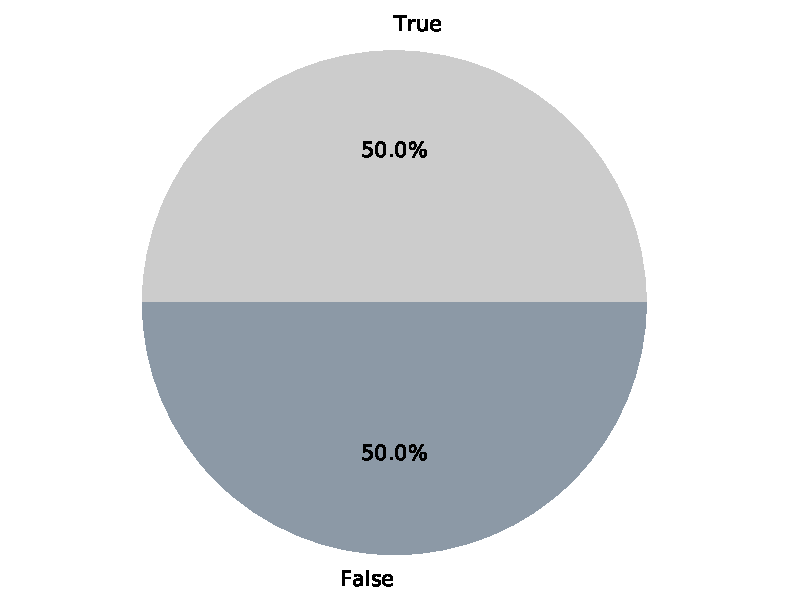
\includegraphics[width=\linewidth]{C:/Users/Laris/Documents/Bachelorarbeit/Git/ThesisPaper/Pictures/hyper_pub.pdf}
		%Lap Top:
		\includegraphics[width=\linewidth]{C:/Users/Larissa/Documents/Uni/Bachelorarbeit/Git/ThesisPaper/Pictures/figure2.pdf}
		\caption{Hyperpartisan Distribution by-Publisher}
	\end{minipage}
	\hspace{.1\linewidth}% Abstand zwischen Bilder
	\begin{minipage}{.45\linewidth}
		%PC:
		%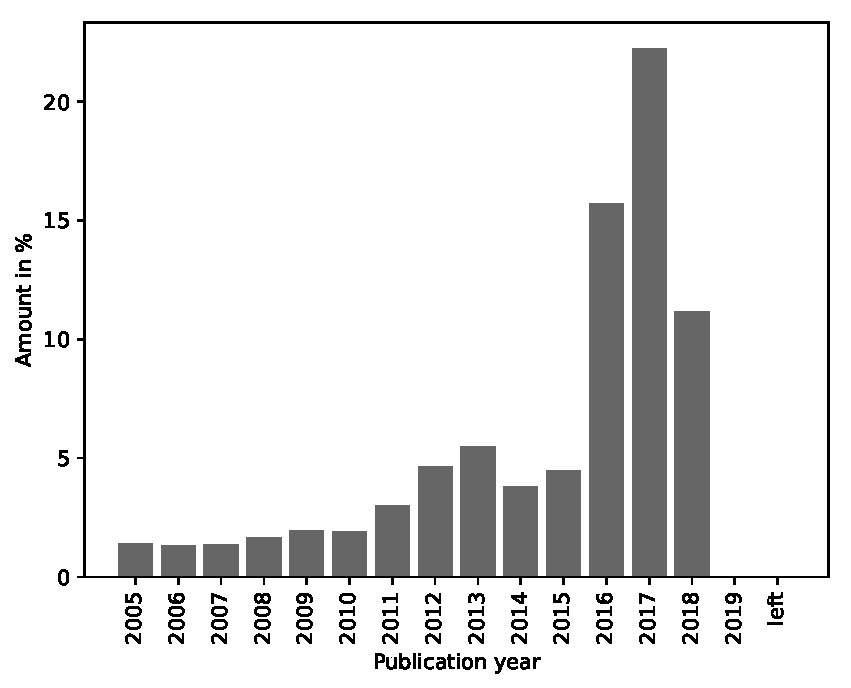
\includegraphics[width=\linewidth]{C:/Users/Laris/Documents/Bachelorarbeit/Git/ThesisPaper/Pictures/histPublisher.pdf}
		%Lap Top:
		\includegraphics[width=\linewidth]{C:/Users/Larissa/Documents/Uni/Bachelorarbeit/Git/ThesisPaper/Pictures/figure.pdf}
		\caption{Publishing Years Distribution by-Publisher}
	\end{minipage}
\end{figure} As mentioned above, this dataset consists of a total of 750,000 articles and is divided into a training record consisting of 600,000 articles and a validation set consisting of 150,000 articles.
The main difference between this dataset and the by-Article labeled one is the type of classification. This is because these articles were not labeled as hyperpartisan based on their content, but due to the publisher (Table 3.1). This likewise influences the distribution of hyperpatisan articles.
 Out of a total of 750,000 items, 375,000 assume the value 'True', while the remaining 375,000 have the value 'False' (Figure 3.1). 
Furthermore, the classification is expressed by the distribution of the additionally contained GroundTruth attribute \textit{Bias}, which informs about the general bias of the publisher. All 375,000 hyperpartisan-labeled articles are assigned to either the left or right sectors, but none are right-centre, least or left-centre and are again 50:50 distributed. The other 50\% are split between the remaining bias, with 'Least' owning the largest share at 37\%.\\
The publicity data is distributed over the years 1964-2018, with most of the data coming from 2012-2018.
%\begin{table}[h]
%	\centering
%	\begin{tabular}{c|c|}
%		\toprule
%		Word & Similarity  \\
%		\midrule
%		obama &0.5890584588050842 \\
%		clinton &0.5385712385177612 \\
%		bannon & 0.5277745127677917 \\
%		priebus &0.5117671489715576 \\
%		hillary & 0.48596829175949097 \\
%		sanders & 0.48391878604888916 \\
%		rubio & 0.4825097918510437 \\
%		\bottomrule
%	\end{tabular}
%\end{table}

\newpage
\section{Dataset labeled by-Article}
\begin{figure}[h]
	\begin{minipage}{.45\linewidth}
		%PC:
		%\includegraphics[width=\linewidth]{C:/Users/Laris/Documents/Bachelorarbeit/Git/ThesisPaper/Pictures/figure2.pdf}
		%Lap Top:
		\includegraphics[width=\linewidth]{C:/Users/Larissa/Documents/Uni/Bachelorarbeit/Git/ThesisPaper/Pictures/figure2.pdf}
		\caption{Hyperpartisan Distribution by-Article}
	\end{minipage}
	\hspace{.1\linewidth}% Abstand zwischen Bilder
	\begin{minipage}{.45\linewidth}
		%PC:
		%\includegraphics[width=\linewidth]{C:/Users/Laris/Documents/Bachelorarbeit/Git/ThesisPaper/Pictures/figure.pdf}
		%Lap Top:
		\includegraphics[width=\linewidth]{C:/Users/Larissa/Documents/Uni/Bachelorarbeit/Git/ThesisPaper/Pictures/figure.pdf}
		\caption{Publishing Years Distribution by-Article}
	\end{minipage}
\end{figure}
The record labeled by-Article consists of a total of 645 articles which were labeled manually. As described in the official SemEval Task 4 paper, each annotator has labeled them using the following scale:
\begin{enumerate}
	\item No hyperpartisan content
	\item Mostly unbiased, non-hyperpartisan content
	\item Not sure
	\item Fair amount of hyperpartisan content
	\item Extreme hyperpartisan content
\end{enumerate}
After that all articles with ratings 1 and 2 were labeled as non-hyperpartisan and all with score 3 and 4 as hyperpartisan.
Accordingly, the hyperpartisan distribution is no longer 50:50, but 36.9\% of all articles were labeled as hyperpartisan and 63.1\% not (Figure 4.3).
\noindent Moreover, in this dataset, the distribution of publication data is not mainly from the years 2012-2018, but from 2016-2018, with the largest number of articles dating back to 2017 at just under 60\% (Figure 4.4). Altogether all 645 articles date from the years 1902-2018.
%This dataset also shows that the feature distribution is different from that of the by-Publisher dataset. For example, here are the most similar words to Trump xxx.
%\begin{table}[h]
%	\centering
%	\begin{tabular}{c|c|}
%		\toprule
%		Word & Similarity  \\
%		\midrule
%		president &0.9992413520812988 \\
%		donald & 0.9992144107818604 \\
%		election & 0.9980630874633789 \\
%		presidential &0.9978925585746765 \\
%		campaign & 0.9978247880935669 \\
%		obama & 0.9977766275405884 \\
%		republican & 0.9974061250686646 \\
%		\bottomrule
%	\end{tabular}
%\end{table}




\chapter{Classification Techniques}
The primary procedure in text classification consist of seven steps \cite{textclassification}. These include  reading the dataset, tokenization, stemming, removing stop words, representing the text using vectors, feature extraction and selection, as well as applying classification algorithms. In the further course of this chapter I  will, therefore describe the steps I took during the development of my program and how they were implemented.

\section{Data Preparation}
In order to be able to work with the existing data in the further course of this project, several preprocessing steps were necessary. In the preprocessing phase of my bachelor's thesis, the data, therefore went through the following steps:
\begin{enumerate}
	\item File Parsing. 
	\item Information Filtering.
	\item Combining Data.
	\item Special Characters and Stop Word Removal.
	\item Tokenization and Stemming.
\end{enumerate}	

\newpage
\subsection{File Parsing}
Since it is difficult to work with the given data in an XML format, the first challenge is to convert these files into a format which allows working with them more easily. The particular challenge here is the size of the dataset labeled by-Publisher. A standard algorithm for reading XML files is provided by pythons library \textit{ElementTree}, called \textit{ElementTree.parse}\cite{parse}. This method returns an ElemenTree type, which is a flexible container object, designed to store hierarchical data structures in memory. Meaning, that this library forms the entire model in the memory which can pose a problem with very large files, such as ours. As a substitute, I therefore use the method \textit{ElemenTree.iterparse}, which can process XML documents in a streaming fashion, retaining in memory only the most recently examined parts of the tree\cite{iterparse}. 


\subsection{Information Filtering}
As mentioned in Chapter 2.1 Data Description, the XML files include various features, which is why it is necessary to extract these from the XML files. In order to do this, the already read content is passed on to an algorithm, where it runs through a double-for-loop. The algorithm checks each item of an element in the content to see which "key" is currently processed. I then save this in an array, so that the features which have already been parsed can be used later. 

\begin{lstlisting}[caption=Parse Ground-Truth File]
def parse_groundtruth(content):
    for event, elem in content:
 	for key, value, in elem.items():
            if key == 'id':
                id_array.append(value)
            elif key == 'hyperpartisan':
                hyperpartisan_array.append(value)
            elif key == 'bias':
                bias_array.append(value)
\end{lstlisting}
\newpage 
\subsection{Combining Data}
Since both, the Groundtruth and Training data contain important information, it is necessary to merge them into one file. I decided to use Python's library \textit{pandas} \cite{pandas} to combine both files into a single one. This, and especially pandas, allows us to read the file more quickly as well as to access individual rows and columns of the merged file in a targeted manner.
\begin{lstlisting}[caption=Merge GroundTruth and Training datasets]
def write_to_csv_articles(title):
    xml_gt = etree.iterparse(path_gt, tag='article')
    xml_training = etree.iterparse(path_training, tag='article')
    content_training = etree.iterparse(path_training, tag='article')
    feature_extraction.parse_features(xml_training)
    groundtruth_parser.parse_groundtruth(xml_gt)
    content = content_parser.parse_content(content_training)

    a_id = feature_extraction.get_id_array()
    published = feature_extraction.get_published_at_array)
    title = feature_extraction.get_title_array()
    bias = groundtruth_parser.get_bias_array()
    hyperpartisan = groundtruth_parser.get_hyperpartisan_array()

    columns = {"ArticleID": a_id,
               "PublishedAt": published,
               "Title": title,
               "Bias": bias,
               "Content": content,
               "Hyperpartisan": hyperpartisan}

    table_frame = Pd.DataFrame(columns)
    table_frame.to_csv(title, encoding='utf-8', index=False)
\end{lstlisting}


\subsection{Special Characters and Stop Word Removal}
Since the GroundTruth and Training datasets have been combined into a single file, the next step  is to remove special characters and stop words. Especially the removal of stopwords is necessary since not all words presented in a document, such as auxiliary verbs, conjunctions and articles \cite{textclassification} are useful for training a classifier.
\begin{lstlisting}[caption=Special Characters and Stop Word Removal]
stop = stopwords.words('english')
df.Content = df.Content.map(lambda x: re.sub(r"[^a-zA-Z0-9]+", ' ', x))
df.Content = df.Content.apply(lambda x: ' '.join([item for item in x.split() if item not in  stop]))
\end{lstlisting}


\subsection{Tokenization and Stemming}
After cleaning the dataset, the words are tokenized in order to convert them into numerical vectors so that a classifier is able to work with them. Tokenization is definied as "the process of demarcating and possibly classifying sections of a string of input characters". The resulting tokens are then passed on to some other form of processing. The process can be considered a sub-task of parsing input.\\
\noindent Stemming is the procedure of reducing the word to its grammatical root. The result is not necessarily a valid word of the language. For example, "recognized" would be converted to "recogniz". Still, the basic word almost always contains the very meaning of the word. Stemming is advantageous in that the algorithm used later now only has to fall back on a few different words instead of many, all of which have the same meaning.\\
\\
\noindent In order to implement Stemming and Tokenization, the \textit{NLTK} \cite{nltk} package provides two functions, due to which only 3 lines of code are necessary.
\begin{lstlisting}[caption=Tokenization and Stemming]
import nltk

df.Content = df.Content.apply(lambda x: ''.join([stemmer.stem(y) for y in x]))
df.Content = df.Content.apply(nltk.word_tokenize)
\end{lstlisting}

\section{Text Representation}
In order for the classifier to be able to work with the text, the first step is to transform the words into a feature vector representation. A document is a sequence of words \cite{word2vecdortmund} so a document can be presented by a One-Hot encoded vector, assigning the value 1 if the document contains the feature-word or 0 if the word does not appear in the document \cite{textclassification}. However, using this technique for word representation resolves in a $V \cdot V$ Matrix, as we have $V$-dimensional vector for each out of $V$ words which can lead to huge memory issues. In addition this does not notion similarity between words. Therefore I will go into further detail for better approaches in the next 2 subchapters.

\subsection{Term Frequency-Inverse Document Frequency}
%\begin{table}[h]
%	\scriptsize
%	\centering
%	\begin{tabular}{cc|cc}
%		\toprule
%		By-Article & \Gls{tfidf} Weight & by-Publisher & \Gls{tfidf} Weight \\
%		\midrule
%		trump & 0.091165 & balls & 0.057251\\
%		bannon & 0.065129 & said & 0.051183 \\
%		president & 0.061829 & medicare & 0.047450 \\
%		kimmel & 0.052415 & martin & 0.046519 \\
%		money & 0.051647 & school & 0.044264\\
%		americans & 0.049132 & university & 0.043572\\
%		people & 0.047342 & says & 0.042079 \\
%		obamacare & 0.042512 & trump & 0.041235\\
%		wall & 0.042117 & carrier & 0.040903\\
%		control & 0.039068 & degree & 0.040704\\
%		\bottomrule
%	\end{tabular}
%	\caption{Top 10 terms by \Gls{tfidf} weight}
%\end{table}
A comparative approach I used in the course of my Bachelor Thesis is Term Frequency - Inverse Document Frequency. Using \gls{tfidf} allows to represent a word as a vector by assigning it weight which is computed through Term-Frequency multiplied with Inverse-Term-Frequency. Table 4.1 shows the 10 terms which have been assigned the highest \gls{tfidf} weights. 
\newpage
Python's library \textit{scikit-learn} \cite{scikit-learn} provides two ways to implement \gls{tfidf} without having to program \gls{tf} and \gls{idf} by itself.
In order to get a generally better overview, I will now explain the 2-step implementation, but note that the class \textit{sklearn.feature\_extraction.text.TfidfVectorizer} enables implementation in just one. \\
\indent Term-Frequency, is a measure that denotes how often a term appears in a document. Inverse Document Frequency, on the other hand, reflects the importance of a term throughout a document corpus. To implement the TF-IDF measure, \textit{scikit-learn} provides the classes \textit{CountVectorizer} and \textit{TfidfTransformer} of the submodule \textit{sklearn.feature\_extraction.text} \cite{tfidf}.
In order to calculate the \gls{tf} measure, the method \textit{fit\_transform()} of the class \textit{CountVectorizer} can be used, which the document corpus is passed as a parameter. \\
\noindent \textit{fit\_transform()} learns a vocabulary dictionary of all tokens and then counts how many times a term \textit{t} occurs in a document \textit{d} and converts the text document into a token matrix.
\noindent The calculation of the \gls{idf}-measure in the second step is similar to the calculation of the \gls{tf}-measure. Again, the method \textit{fit\_transform()} is called. In contrast to the method of the \textit{CountVectorizer}, the text document is no longer passed as a parameter, but the token matrix of \textit{CountVectorizer}. \\
\indent It should be noted that the shape of the finalized \gls{tfidf} matrix depends on the document corpus. The first time the conversion is carried out, the two objects of the respective classes learn the respective vocabulary through the keyword \textit{"fit\_"}. If a second text document should be converted to \gls{tfidf} vectors afterwards, which is supposed to be used in connection with the already converted text document, it is necessary to use the same \textit{CountVectorizer} and the same \textit{TfidfTransformer}. This is, because otherwise the error message "Dimension Mismatch" would appear in later prediction calls.
Let's take the following example: \\
\noindent If the two datasets labeled by-Aticle and publisher are converted with the same \textit{CountVectorizer} and \textit{TfidfTransformer}, we obtain the following dimensions:
\begin{itemize}
	\item By-Publisher: (600000, 708863)
	\item By-Article: (645, 708863)	
\end{itemize}
\newpage
\noindent If the two methods \textit{fit\_transform()} were called for both datasets, \textit{CountVectorizer} and \textit{TfidfTransformer} would be initialized each time, which would result in the following dimensions:
\begin{itemize}
	\item By-Publisher: (600000, 708863)
	\item By-Article: (645, 11485)	
\end{itemize}
\begin{lstlisting}[caption=\gls{tfidf}]
def tf_idf_forContent(content):
count_vect = CountVectorizer()
tfidf_transformer = TfidfTransformer()

content_counts = count_vect.fit_transform(content)
content_tfidf = tfidf_transformer.fit_transform(content_counts)

return content_tfidf
\end{lstlisting}

\newpage
\subsection{Word2Vec} 
%\begin{table}[h]
%	\scriptsize
%	\centering
%	\begin{tabular}{cc|cc}
%		\toprule
%		By-Article & Similarity  & by-Publisher & Similarity \\
%		\midrule
%		president & 0.9992413520812988 & obama & 0.5890584588050842 \\
%		donald & 0.9992144107818604 & clinton & 0.5385712385177612 \\
%		election & 0.9980630874633789 & bannon & 0.5277745127677917 \\
%		presidential & 0.9978925585746765 & priebus & 0.5117671489715576 \\
%		campaign & 0.9978247880935669 & hillary &  0.48596829175949097 \\
%		\bottomrule
%	\end{tabular}
%	\caption{Most similar word to 'trump'}
%\end{table}
For a further comparison and an approximation to the classification model used ater on, I did not only use \gls{tfidf} as a vector representation method as part of my Bachelor Thesis, but also word embeddings - especially the \textit{word2vec} model. \\
Word2Vec represents words as vectors. Unlike the  \gls{tfidf} method, however, not only word frequencies and priorities are considered but also the connection of individual words to others. Again, several methods of implementation exist. 
\noindent As part of my Bachelor Thesis, I decided to use  the library \textit{gensim} \cite{gensim} to implement my Word2Vec model. With \textit{gensim} it is  possible to do  unsupervised semantic modelling from plain text. This makes it possible to implement a Word"vec model using only a few lines of code without having to program Skip-Gram of \gls{cbow} yourself. 
 Algorithm 7 shows that the implementation of the model is straightforward, as it is pretty much the only step we need to program. By default, \textit{gensim} uses \gls{cbow} which can be  changed  by adding the following parameter to the parameters list: \textit{sg=1}. As for the other parameters, 18 more exist which can be viewed at the official \text{scikit-learn} page \footnote{https://radimrehurek.com/gensim/models/word2vec.html}, but I decided to focus only on the important ones. \textit{Vocab} is our text corpus, which needs to be transformed into a list of tokenized sentences. \textit{Size} determines the dimension of the word vectors, \textit{window} the maximum distance between the current and predicted word within a sentence, \textit{min\_count}  how often a word must appear to be included in the vocabulary and \textit{iter} how many iterations  should be performed on the corpus. What exactly happens here is that a neural network with a single hidden layer is trained to predict the current word based on the context. The resulting vector consists of several features that describe the target word.
 \begin{lstlisting}[caption=Word2Vec with gensim]
 model = gensim.models.Word2Vec(vocab, min_count=10, window=10, size=300, iter=10)
 \end{lstlisting}
\indent 
After the model has been trained it is possible to get information about the similarity of two words by calling the method $model.wv.similarity(word_1, word_2)$. Table 4.2 shows the 6 most similar words to "trump" of both datasets. This is possible by calculating the cosine similarity of two words in the vector space. As the range of the cosine similarity can go from [-1 to 1], words that are completely the same are assigned the value \textit{1} and words that are not similar at all are given the value \textit{-1}. 
\newpage
\indent The resulting word vectors now have the dimension defined in the parameter \textit{size}. In order to be able to form features from them, I averaged the word ebeddings of all words in a sentence (algorithm 8).
\begin{lstlisting}[caption=sent\_vectorizer]
def sent_vectorizer(sent, model):
    sent_vec = []
    numw = 0
    for w in sent:
        try:
            if numw == 0:
                sent_vec = model[w]
            else:
                sent_vec = np.add(sent_vec, model[w])
            numw += 1
        except:
            pass

    return np.asarray(sent_vec) / numw
\end{lstlisting}

\section{Classification Methods}
The given classification task in this thesis is of binary nature. Given a set of articles, it should be determined whether or not an article is hyperpartisan. For training different classifiers I used different approaches. \\

\subsection{Classical Approach}
In the first approach, the first step I performed was representing the articles using Word Embeddings and \gls{tfidf} Measure. The word2vec, TfidfTransformer and CountVectorizer were both trained on the by-Publisher dataset, since it contains 600.000  articles and, therefore, has more data to train these models. In the second step I did a GridSearch to get the optimal parameters for the classifiers based on the given datasets, whereupon in the third step, I performed training using the classifiers Multinomial Naive Bayes, Logistic Regression and Random Forest on the datasets labeled by-Article and by-Publisher. For the implementation of these classifiers I used Python's library scikit-learn, which makes it possible to use already implemented classifiers without having to program them from scratch. Here a classification algorithm is a Python object, which represents an estimator for classifications and implements the methods fit() and predict(). The aim is that the classifier instance learns from the defined model by passing the training dataset to the method fit().
\newpage
\indent A simple implementation of GridSearch is provided by \textit{scikit-learn} through the class \textit{sklearn.model\_selection.GridSearchCV} \cite{codegridsearch}. This class evaluates all possible combinations of parameters when calling the method \textit{fit()} and keeps the best combination. The parameters that can be passed to the class include \textit{estimator}, which specifies the classifier, \textit{param\_grid}, which is the parameter set, \textit{scoring}, which specifies the measure to evaluate the test set, and \textit{cv} to determine how many cross-validation splits must be performed. \\
%begin{algorithm}[H]
%	\DontPrintSemicolon
%	from sklearn.model\_selection import GridSearchCV\;
%	from sklearn.naive\_bayes import MultinomialNB\;
%	\BlankLine
%	parameter\_candidates = \{'alpha': np.linspace(0.5, 1.5, 6), 'fit\_prior': [True, False]\}\;
%	clf = GridSearchCV(estimator=MultinomialNB(), param\_grid=parameter\_candidates, scoring='accuracy', cv=10)\;
%	clf.fit(features, labels)\;
%	\caption{Grid Search for \gls{mnb} classifier}
%\end{algorithm}
\indent The Multinomial Naies Bayes classifier is an estimator for classifying multinomial distributed data. For implemening the Naives Bayes model scikit-learn provides the class \textit{sklearn.naive\_bayes.MultinomialNB} \cite{codemulinomialnb} and classifies as follows:
\[
\hat{\Theta}_{yi}=\frac{N_{yi}+\alpha}{N_y + \alpha n}
\]

\noindent Here $\Theta$ is estimated by a smoothed version of the maximum likelihood, $N_{yi}=\sum_{x \in T}x_i$ is the number of times a feature $i$ appears in a sample of class $y$ in the training set, $N_y=\sum_{i=1}^{n}N_{yi}$ is the total count of all features for class $y$ and $\alpha$ incorporates the smoothing parameter due to which zero probabilities will be prevented.
The \textit{MultinomialNB} classifier includes the parameters \textit{alpha}, \textit{fit\_prior} and \textit{class\_prior}, where \textit{alpha} specifies the smoothing value, \textit{fit\_prior} whether the class probalilities should be learned in advance and \textit{class\_prior} specifies the prior probabilities of the classes.\\
\indent The Random Forest Classifier is a classification technique that creates multiple decision trees from randomly selected subsets of training data. For implementing the Random Forest Classifier, \textit{scikit-learn} provides the class \textit{sklearn.ensemble.Ran-domForestClassifier} \cite{coderandomforest}. Unlike the original publication \cite{randomforest}, the \textit{scikit-learn} classifier determines the final class by averaging the probabilistic forecasts as opposed to having each classifier vote in favour of a solitary class. The Random Forest classifier includes 17 parameters, of which I have included \textit{n\_estimators}, criterion, max\_depth, min\_samples\_leaf, max\_features and bootstrap. Here, n\_estimators determines the number of trees in the forest, \textit{criterion} which impurity measure to utilize, \textit{max\_depth} determines the maximum depth of a tree, \textit{min\_samples\_leaf} determines the base number of samples to be at a leaf node, \textit{max\_features} the quantity of features that must be considered in the search for the best partition and \textit{bootstrap} indicates whether bootstrap models are utilized when making trees.\\
\indent The Logistic Regression classifier is a model for classification, where the probabilities depicting the potential results of a solitary class are modelled utilizing a logistic function. The provided classifier of \textit{scikit-learn} offers the possibility not only to classify binary, but also One-vs-Rest and multinomial. There are several solvers available for this, yet since our classification problem only refers to binary classification, I will only discuss those aspects of the logistic regression classifier in the following section. Scikit-learns Logistic Regression Classifier provides L1, L2 and Elastic-Net Regularization \cite{logisticregression}. As solvers, \textit{liblinear}, \textit{newton-cg}, \textit{lbgfs}, \textit{sag} and \textit{saga} are available. \textit{Scikit-learn} points out, that \textit{liblinear} is a good algorithm for small datasets, whereas \textit{sag} and \textit{saga} are faster for large datasets. 
\newpage \noindent Also, \textit{newton-cg}, \textit{lbgfs} and \textit{sag} only handle \textit{L2} penalty, whereas \textit{liblinear} also handles \textit{L1} penalty and \textit{saga} in addition \textit{elasticnet}. \textit{Liblinear} uses a coordinate descent algorithm, the \textit{sag} solver a Stochastic Average Gradient descent, \textit{saga} is a variant of \textit{sag} and therefor supports the non-smooth penalty \textit{L1} and \textit{elasticnet} and the \textit{lbfgs} solver is an optimization algorithm that approximates the Broyden–Fletcher–Goldfarb–Shanno algorithm.\\


\subsection{Novel Approach using Bidirectional Encoder Representations from Transformers}
In the second approach of my classification I used Google's model for Bidirectional Encoder Representations from Transformers. Here I do not pre-train the model like the Clint Buchanan group, but use the already pre-trained models and fine-tune using the data sets labeled by-Article and by-Publisher. Meanwhile many possibilities exist to use the Bert model, including TensorFlow Hub or a PyTorch \cite{pytorch} interface, whereby in this thesis the original GitHub Code was used.\\
\indent In the official github repository \footnote{\url{https://github.com/google-research/bert}}  both models, \gls{bert}$_{Base}$ and \gls{bert}$_{Large}$, were published. This includes the TensorFlow \cite{tensorflow} code, pre-trained checkpoints for both lowercase and uppercase versions of \gls{bert}$_{Base}$ and \gls{bert}$_{Large}$, as well as the TensorFlow code for replication of the most important fine-tuning experiments from the paper. The existing pre-trained models consist of a \textit{.zip} file, which contains the TensorFlow checkpoint for initializing the pre-trained weights, a vocab file to map WordPiece to word id, as well as a config file, which describes the hyperparameters of the model. \\ 
\indent A total of 15 python files have been published on GitHub, of which \textit{\_\_init\_\_.py}, \textit{modeling.py}, \textit{optimization.py}, \textit{tokenization.py} and \textit{run\_classifier.py} are required for classification tasks. Here \textit{run\_classifier.py} is the main file which has to be executed in order to perform fine-tuning and consists of the fine-tuning code for the \gls{bert} model, as well as various classes. These different classes have been implemented specifically for the tasks mentioned in the paper and specify how to access the training, development and test data, which labels exist and creates the input examples for the \gls{bert} model. Since these classes have to be implemented in a differentiated way, it is therefore necessary to implement a separate class, which can be used within the framework of the data sets available in this thesis. However, it is largely possible to fall back on already implemented classes. For example, of the \textit{ColaProcessor} class, only the methods \textit{ create\_examples} (Algorithm 14) as well as get\_labels must be modified. 
\newpage
\begin{lstlisting}[caption=Create\_examples in BERT]
def _create_examples(self, lines, set_type):
    """Creates examples for the training and dev sets."""
    examples = []
    for (i, line) in enumerate(lines):
        if i == 0:
            continue
        guid = "%s-%s" % (set_type, line[0])
        text_a = line[1]
        label = line[2]
        examples.append(InputExample(guid=guid, text_a=text_a, text_b=None, label=label))
    return examples
\end{lstlisting}
\indent A slightly modified version of the combined GroundTruth- and Training datasets will be passed to this new class, as only the article's content, IDs and labels for the input examples to be generated are required. Since BERT uses \textit{.tsv} as the default file format, it is also necessary to save the modified file in this form. \\
\noindent The execution of the \textit{run,\_classifier.py} file includes additional passing of 12 arguments (Listing 5.2), where \textit{train\_batch\_size}, \textit{learning\_rate} and \textit{num\_train\_epochs} represent the model's hyperparameters. 

\indent In a  single training epoch, the entire data set is passed through a neural network once. Hereby, a higher number of epochs is required to avoid under-fitting due to a small number of updated weights. However, too many epochs may lead to over-fitting. In the paper, the authors state, that a number of  3 or 4 epochs worked best across different tasks. I experienced that a number of 10 epochs slightly improved the model when trained on the Publisher record, while it made no real difference on the Article record. This is different from the paper, which states that the result with different parameters should not vary as much on large as on small dataset.  \\
\indent Since it is not possible to transfer an entire data set into a neural network at once, batch size defines the total number of training examples contained in a single batch. Here, the paper refers  to an optimal number of 16 or 32. On the official GitHub page, however, it is pointed out that all experiments in the paper were fine-tuned on a cloud-TPU with 64GB RAM and using the same hyperparameters  on a GPU with 12 to 16GB RAM may lead to out-of-memory issues. Therefore in the same section, the maximum batch size for an associated sequence length and the associated Bert model is mentioned, whereas for the \gls{bert}$_{Base}$ model with a sequence length of 512 the corresponding maximum batch size is 6. However, on
a GPU with 12GB RAM, I  experienced that using a batch size larger than 2 is not possible on the by-Publisher labeled data set. Despite this, I decided not to use a smaller sequence length, since a length of 512 is already not enough for a complete article. 
\newpage
\begin{lstlisting}[caption=run\_classifier prompt with FLAGS]
export BERT_BASE_DIR=/path_to_bert_model/uncased_L-12_H-768_A-12
export DATA_DIR=/path_to_input_data/

python run_classifier.py \
--task_name=ba \
--do_train=true \
--do_eval=true \
--data_dir=$DATA_DIR \
--vocab_file=$BERT_BASE_DIR/vocab.txt \
--bert_config_file=$BERT_BASE_DIR/bert_config.json \
--init_checkpoint=$BERT_BASE_DIR/bert_model.ckpt \
--max_seq_length=512 \
--train_batch_size=2 \
--learning_rate=3e-5 \
--num_train_epochs=4.0 \
--output_dir=/path_for_output_data/
\end{lstlisting}
\indent Learning rate tells the optimizer of a neural network how far it is supposed to set the weights in the opposite direction to the gradient for a mini batch. If the learning rate is low, training is more reliable, but  optimization will take a lot more time, whereas with a high learning rate, the training may not approach or even diverge. The authors of the paper refer to an optimal learning rate in relation to the Adam gradient \cite{adam} of 5e-5, 3-5 or 2-5. I trained the model with the parameters 5e-5, 3e-5, 2-5 and 1e-5 and the model produced the best results on both data sets with the learning rate 2e-5. 

\chapter{Evaluation}
The evaluation based on the test data set is hosted on TIRA \cite{tira}. TIRA is an "Evaluation as a Service" \cite{evaluationasaservice} and focuses on hosting common tasks to facilitate the delivery of software. Because of TIRA, it is not possible to gain insight into the test data set in order not to influence the result.
In order to test the classifiers on the test dataset, the organizers of the competition provided me with a virtual machine in TIRA. It is only possible to access the test data within the TIRA interface. To run the software, a shell-command must be passed in this interface, which contains the Python program, the path to the directory of the test dataset and the path for the output. In this connection, it was necessary that the passed file creates a .txt file as output, which consists of one column for the ID of the article and one column for the prediction. \\
\indent It is then possible to forward the run to the evaluation software, which then outputs Accuracy, Precision, Recall and F1-Score. When evaluated on the test data, the results are not immediately visible, but have to be unblinded by the organizers. 
\begin{figure}[h]
	\centering
	%PC:
	%\includegraphics[width=0.8\linewidth]{C:/Users/Laris/Documents/Bachelorarbeit/Git/ThesisPaper/Pictures/tira3.png}
	%Lap Top:
	\includegraphics[width=0.8\linewidth]{C:/Users/Larissa/Documents/Uni/Bachelorarbeit/Git/ThesisPaper/Pictures/tira3.png}
	\caption{TIRA Interface}
\end{figure}


\begin{table}[t]
	\centering
	\begin{tabular}{c|c|c|c|c}
		\toprule
		Classifier & Accuracy & Precision & Recall &F1  \\
		\midrule
		Best score of all teams & 0.822 & 0.883 & 0.971 & 0.821 \\
		\midrule
		Logistic Regression-Article$_{TFIDF}$ & 0.732 & 0.770 & 0.662 & 0.712 \\
		Logistic Regression-Article$_{WB}$ & 0.692 & 0.692 & 0.694 & 0.693 \\
		Logistic Regression-Publisher$_{TFIDF}$ & 0.622 & 0.579 & 0.901 & 0.705 \\
		Logistic Regression-Publisher$_{WB}$ & 0.600 & 0.559 & \textbf{0.949} & 0.704 \\
		Random Forest-Article$_{TFIDF}$ & 0.622 & \textbf{0.79} & 0.334 & 0.47 \\
		Random Forest-Article$_{WB}$ & 0.75 & 0.785 & 0.688 & \textbf{0.733} \\
		Random Forest-Publisher$_{TFIDF}$ & \textbf{0.772} & 0.775 & 0.767 & 0.771 \\
		Random Forest-Publisher$_{WB}$ & 0.646 & 0.593 & 0.93 & 0.725 \\
		\gls{mnb}-Article$_{TFIDF}$ & 0.575 & 0.747 & 0.226 & 0.437 \\
		\gls{mnb}-Publisher$_{TFIDF}$ & 0.635 & 0.584 & 0.939 & 0.720 \\
		BERT-Article & 0.705 & 0.25 & 0.028 & 0.05 \\
		BERT-Publisher & 0.380 & 0.306 & 0.944 & 0.459 \\
		\bottomrule
	\end{tabular}
	\caption{Evaluation Results -- Article: Classifier has been trained on the by-Article dataset; -Publisher: Classifier has been trained on the by-Publisher dataset; -WB: Word Embeddings have been used; -TFIDF: \gls{tfidf}}
\end{table}
\newpage
For the evaluation I used different models for comparison. A total of 12 types of classifiers were used for comparing different methods of classification. Among these, each classifier mentioned in Chapter 5 was trained on the by-Article and on the by-Publisher datasets, as well as each of these using \gls{tfidf} and Word Embeddings to represent the article. As a final comparison step, the \gls{bert} model was taken in to see if it stands out from the classical classifiers. Table 6.1 shows the results. The results refer to the evaluation on the test data set labeled by-Article, as this was the basis for the results of the competition. \\
\indent As a comparison to the scores of the other teams, the Accuracy measure is considered, since this was the main measure in relation to the competition. It turns out that the Random Forest Classifier which was trained on the basis of  the \gls{tfidf} measure and the by-Publisher labeled data set, performed best with an Accuracy score of 0.772, which would result in 10$^{th}$ place out of 42 teams in the competition.\footnote{Leaderboard: https://pan.webis.de/semeval19/semeval19-web/leaderboard.html} In comparison, the winners achieved a score of 0.822.\\
\indent Overall, the text representation was better with Word Embeddings than with the \gls{tfidf} measure. This can be explained by the fact that word embeddings include semantic connections, which plays an important role in text classification. \\
\indent It can also be seen that the classifiers performed better when they were trained on the by-Article labeled data set than on the by-Publishers ones. This is probably due to the fact that this record contained more accurate hyperpartisan features than the by-Publisher ones. I therefore suspect that the classifiers would have done even better, if a hand-labeled dataset with the size of the by-Publisher labeled record had been available. 
\newpage
\indent Interestingly enough, the \gls{bert} model trained on the by-Publisher dataset performed astonishingly poor, with having an Accuracy score of 0.38. The Accuracy score of the \gls{bert} model, which was trained on the basis of the dataset labeled by-Article, scores 0.705, quite similar to the Bertha von Suttner group, who reached a score of 0.771. This shows that it makes sense to pre-train the BERT model on the basis of the available data sets and not only to fine-tune it on the basis of the pre-trained models. 

\chapter{Conclusion}
The goal of this Bachelor Thesis was to develop a program that allows to recognize if a news article is hyperpartisan or not. Two different approaches were used. In the first one classical classification techniques were used. These included word embeddings using word2vec and the Term Frequency-Inverse Term Frenquency measure for the machine representation of an article as well as Multinomial Naive Bayes, Logistic Regression and Random Forest for classifying. As a second approach I used the \gls{bert} model by fine-tuning on the by-Article labeled dataset based on the pre-trained BERT models. \\
\indent It turned out among the classical approaches that it plays a role to what extent the article was represented. In contrast to \gls{tfidf}, Word Embeddings thus not only deal with word frequencies and priorities, but also with semantic features. In this context it is not surprising that the group "Vernon Fernwick" from the competition reaches second place by including handmade features. \\
\indent In addition, it turned out that the quality of the labels plays a special role. The data record labeled by-Publisher, performed poorer than the data record labeled by Article. This is probably due to the fact that the publisher's dataset, was not labeled by hand, and also contains articles which were labeled as hyperpartisan when they were not. This leads to a wrong learning of features.\\
\indent The newly used BERT approach did not improve the performance of the classification within the scope of this classification task. The model trained on the publisher dataset came off surprisingly bad with an Accuracy of 0.38. However, the Clint Buchanan group showed that the \gls{bert} model can achieve better performance by using different implementation approaches.\\
\indent Overall, it can be said that the classifiers described here, as well as those of the competition, produced good results. This suggests that it is quite feasible to use computers to recognize hyperpartisan articles and support people in doing so.
An approach as to how such a classifier could be used would be to integrate it into the Internet browser as an add-on. This could show people from the beginning whether an article is likely to be hyperpartisan or not. This would possibly influence their opinion about this article, whereupon spreading of fake news might decrease.


\bibliography{BA}{}
\bibliographystyle{plain}
\pagestyle{empty}

\newpage
\section*{Ehrenw\"ortliche Erkl\"arung}
Ich versichere, dass ich die beiliegende Bachelorarbeit ohne Hilfe Dritter
und ohne Benutzung anderer als der angegebenen Quellen und Hilfsmittel
angefertigt und die den benutzten Quellen w\"ortlich oder inhaltlich
entnommenen Stellen als solche kenntlich gemacht habe. Diese Arbeit
hat in gleicher oder \"ahnlicher Form noch keiner Pr\"ufungsbeh\"orde
vorgelegen. Ich bin mir bewusst, dass eine falsche Erkl\"arung rechtliche Folgen haben
wird.
\\
\\

\noindent
Mannheim, den 02.07.2019 \hspace{4cm} Unterschrift


\end{document}
